% =====================================================================
%  main.tex  --  IEEEtran conference paper
%  Verifiable Identity and Delegation for Orchestrated Multi-Agent
%  AI Systems: A Blockchain-Anchored Framework
%
%  HOW TO USE IN OVERLEAF
%  1. New Project -> Upload Project, or create a blank project and add:
%       main.tex, references.bib,
%       fig_arch.png, fig_flow.png, results_fig.png
%  2. Set the compiler to pdfLaTeX (Menu -> Compiler -> pdfLaTeX).
%  3. Recompile. Overleaf runs bibtex automatically; if references look
%     empty on the first run, just hit Recompile once more.
%
%  The IEEEtran class + IEEEtran.bst are built into Overleaf, so the
%  formatting (two columns, headings, reference style) is handled for you.
% =====================================================================
\documentclass[conference]{IEEEtran}

\usepackage{graphicx}
\usepackage{amsmath,amssymb}
\usepackage{algorithm}
\usepackage{algpseudocode}
\usepackage{booktabs}
\usepackage{array}
\usepackage{pifont}
\usepackage{url}
\usepackage[T1]{fontenc}
\usepackage{cite}

% check / cross marks for the capability table
\newcommand{\cmark}{\ding{51}}
\newcommand{\xmark}{\ding{55}}

\begin{document}

\title{Verifiable Identity and Delegation for\\Orchestrated Multi-Agent AI Systems:\\A Blockchain-Anchored Framework}

\author{%
\IEEEauthorblockN{P Anand Kumar}
\IEEEauthorblockA{Dept. of Computer Science and Engineering\\
Chennai Institute of Technology\\
Chennai, Tamil Nadu, India\\
panandkumar.cse2024@citchennai.net}
}

\maketitle

\begin{abstract}
AI agents now act for users and organizations: they plan, call tools, and carry out consequential actions with little human oversight. Most multi-agent platforms still identify these agents with a static allow-list of names, which can say only whether a name is known. It cannot prove who actually acted, who authorized them, or whether the action stayed within the authority they were given. We present a framework that gives each agent a decentralized identifier (DID) and turns every orchestrator-to-specialist hand-off into a signed, revocable delegation credential anchored on a permissioned ledger. Three smart contracts---an Identity Registry, a Delegation Registry, and a Revocation and Policy contract---record the grants and the action attestations, and a Model Context Protocol (MCP) layer runs an action only after its full authority chain verifies on-chain. We built the authorization layer with Ed25519 identities and signed credentials and tested it against two baselines, one with no blockchain and one using an allow-list, across five attack scenarios. It blocks every spoofed, out-of-scope, revoked, expired, and replayed action that both baselines let through, rebuilds the complete authority chain for all executed actions, and adds about 0.24~ms of cryptographic work per decision---a small fraction of the ledger anchoring cost.
\end{abstract}

\begin{IEEEkeywords}
Blockchain, multi-agent systems, decentralized identity, verifiable credentials, AI agents, delegation, Model Context Protocol, smart contracts, auditability.
\end{IEEEkeywords}

% =====================================================================
\section{Introduction}
Large language models started as passive responders. They are now agents: they plan, call external tools, and act with little human supervision. A common production pattern puts a central orchestrator in charge of a goal, which it breaks into subtasks and hands to specialist agents, each owning one narrow job such as risk scoring, fraud screening, or payment execution. These agents write code, move data, and trigger transactions in milliseconds. None of the friction a human login or a manual review would add is present.

That speed comes with an identity and accountability gap. An agent has no legal identity, cannot be held responsible, and is trivial to impersonate. Enterprises already run more non-human identities---bots, devices, agents---than human ones, yet inside most multi-agent platforms an agent is identified by nothing more than its name on an allow-list. A name on a list answers one question: is this name known? The questions that matter for a delegated action go unanswered. Is the agent cryptographically who it claims to be? Did the orchestrator authorize this specific action? Was that authority still valid when the action ran? And can the whole chain of authority be reconstructed afterwards for an audit?

Some recent systems pair a blockchain with agentic AI to make actions auditable and to check policy before anything runs \cite{jan2025}. They show that a permissioned ledger can record an agent's perception--reasoning--action cycle and turn away unsafe actions. But they still authenticate agents with a whitelist, and they model neither delegated authority nor its revocation. A parallel line of work on the ``agent economy'' \cite{xu2026} and on payment authorization for autonomous agents \cite{tiva2025} makes the case that agents need on-chain decentralized identity, but it is aimed at economic settlement, not at the delegation that happens inside an orchestrated system.

This paper closes that gap. We treat each agent as a cryptographic principal in its own right, and we treat every orchestrator-to-specialist hand-off as an explicit, scoped, revocable delegation credential on a permissioned ledger. An action runs only when its full authority chain---root user to orchestrator to specialist---verifies on-chain at the moment of execution. Our contributions are:

\begin{enumerate}
\item A cryptographic identity scheme for agents in orchestrated systems, replacing allow-list names with DID-bound keys.
\item A verifiable delegation protocol that records scoped, time-bounded, revocable grants on a permissioned ledger and ties every executed action to its authority chain.
\item A smart-contract enforcement layer---Identity Registry, Delegation Registry, and Revocation/Policy contracts---wired into a Model Context Protocol (MCP) execution layer, so only verifiable actions run.
\item A working implementation of that layer and an evaluation over five attack scenarios against no-blockchain and allow-list baselines, with measured spoofing resistance, auditability, revocation latency, and overhead.
\end{enumerate}

Section~\ref{sec:bg} covers the primitives we build on. Section~\ref{sec:rel} places the work against prior research. Section~\ref{sec:fw} gives the framework, threat model, delegation protocol, and contract logic. Section~\ref{sec:exp} describes the implementation and how we evaluated it, Section~\ref{sec:res} reports the measured results, and Section~\ref{sec:sec} works through the security argument threat by threat. Section~\ref{sec:concl} concludes.

% =====================================================================
\section{Background}\label{sec:bg}
\subsection{Orchestrated Multi-Agent Systems}
Agents that reason and act interleave deliberation with tool calls \cite{react2023}. Modern platforms stack several of them under a central orchestrator, which splits a user goal into sub-goals and routes each to a specialist that owns one capability and may reach out to external tools. A broad survey of LLM-based agents \cite{wang2024survey} tracks how fast this pattern has spread, but it treats trust between agents as an application detail rather than a security primitive. We take the opposite view.

\subsection{Decentralized Identifiers and Verifiable Credentials}
A decentralized identifier (DID) \cite{w3c-did} is a globally unique identifier that resolves to a document of public keys, with no central registrar. A verifiable credential (VC) \cite{w3c-vc,sporny2019} is a signed, tamper-evident statement about a subject. Both were built for people and organizations---and underpin regulatory identity efforts such as eIDAS~2.0 \cite{eidas2024}---but they fit software agents just as well: a DID names the agent, and a VC says what it may do. We use a signed VC-style object as the on-chain delegation credential and a DID registry as the identity anchor.

\subsection{Digital Signatures}
Each identity is an Ed25519 key pair \cite{ed25519,rfc8032}---the Edwards-curve signature scheme, chosen for fast verification and 128-bit security. An agent signs both its credentials and the actions it proposes. Checking that signature against the registered public key is exactly what tells a real agent apart from an impostor, and it is exactly what a name-based allow-list cannot do.

\subsection{Permissioned Ledgers and Smart Contracts}
A permissioned ledger such as Hyperledger Fabric \cite{fabric2018} keeps an append-only, tamper-evident record across a known set of endorsing peers and runs deterministic chaincode. Compared with public chains \cite{nakamoto2008,wood2014}, it gives up open decentralization in exchange for higher throughput and privacy---the right trade for an enterprise deployment, much as globally distributed transactional databases \cite{spanner2013} trade openness for consistency and performance. We use it to anchor credential and action hashes, which fixes the existence, scope, and timing of every grant in an auditable form.

\subsection{The Model Context Protocol}
The Model Context Protocol (MCP) \cite{mcp2024} is a standard way for agents to reach tools and data. Every consequential external effect passes through an MCP connector, which makes that connector the natural checkpoint for authorization: a tool runs an action only after its authority chain verifies.

% =====================================================================
\section{Related Work}\label{sec:rel}
\subsection{Blockchain-Governed Agentic AI}
The closest prior system runs a multi-agent reasoning stack on a permissioned blockchain, validating each proposed action with smart contracts before it executes and recording it immutably \cite{jan2025}. It uses a perception--reasoning--action pipeline, Hyperledger Fabric for governance, and MCP for actuation, and reports that on-chain validation stops unsafe actions for a modest latency cost. The weakness is identity: an agent is just a whitelist entry, and the model has no way for one agent to hand bounded authority to another, let alone to revoke it. We keep the pre-execution checks and the audit trail of \cite{jan2025}, but swap the whitelist for cryptographic DIDs and make scoped, revocable delegation the central abstraction.

\subsection{Decentralized Identity and Verifiable Credentials}
DIDs \cite{w3c-did} and VCs \cite{w3c-vc} give a W3C-standard basis for tamper-evident identity and authorization without one central authority. Early blockchain-for-identity systems \cite{zyskind2015} showed a ledger could govern access to personal data. These primitives were built for people and organizations, but they carry over to software agents cleanly. We use them directly, with a signed VC-style object as the on-chain delegation credential.

\subsection{Autonomous-Agent Economies and Authorization}
Several groups argue that autonomous agents need native on-chain infrastructure. The agent-economy proposal \cite{xu2026} outlines a layered design where agents hold sovereign DIDs, build reputation, and settle payments through account abstraction \cite{erc4337}. Intent-verification work for agent payments \cite{tiva2025} gives each agent a DID and a delegation credential and checks on-chain that a transaction matches authorized intent. We share their use of DIDs and delegation, but they target machine-to-machine commerce; the delegation chains inside an orchestrated task-execution platform are ours to handle.

\subsection{Access Control and Delegation}
Role-based access control \cite{rbac1996} has long governed what principals may do, and delegation is a well-studied problem in distributed systems. Our angle is to express delegation between agents as a chain of signed credentials whose scope only narrows, anchored on a ledger and checked at the MCP boundary---so authority is enforceable before an action and reconstructable after it.

\subsection{Summary of the Gap}
No existing system, across any of these lines, offers cryptographic, scoped, and revocable delegation for orchestrated multi-agent action with on-chain auditability tied to execution. Table~\ref{tab:cap} lays the capabilities side by side; our framework fills the empty column.

\begin{table}[t]
\centering
\caption{Capability Comparison of Agent-Authorization Approaches}
\label{tab:cap}
\renewcommand{\arraystretch}{1.25}
\begin{tabular}{@{}lccc@{}}
\toprule
\textbf{Property} & \textbf{B0 None} & \textbf{B1 Allow-list} & \textbf{B2 Ours}\\
\midrule
Cryptographic identity      & \xmark & \xmark & \cmark\\
Scoped delegation           & \xmark & \xmark & \cmark\\
Revocation                  & \xmark & \xmark & \cmark\\
Pre-execution enforcement   & \xmark & \cmark & \cmark\\
Execution-bound audit trail & \xmark & \cmark & \cmark\\
Chain reconstruction        & \xmark & \xmark & \cmark\\
\bottomrule
\end{tabular}
\end{table}

% =====================================================================
\section{Proposed Framework}\label{sec:fw}
\subsection{Architecture Overview}
The framework splits into four planes, shown in Fig.~\ref{fig:arch}. The Identity Plane holds a Passport (issuer) service that mints credentials and an Identity Registry that maps each agent DID to its public key. The Orchestration Plane holds the root authority---the user or organization---the orchestrator, and the specialist agents. The Governance Plane is a permissioned ledger running three smart contracts. The Execution Plane uses MCP connectors to call external tools and to anchor an attestation once an action finishes.

\begin{figure}[t]
\centering
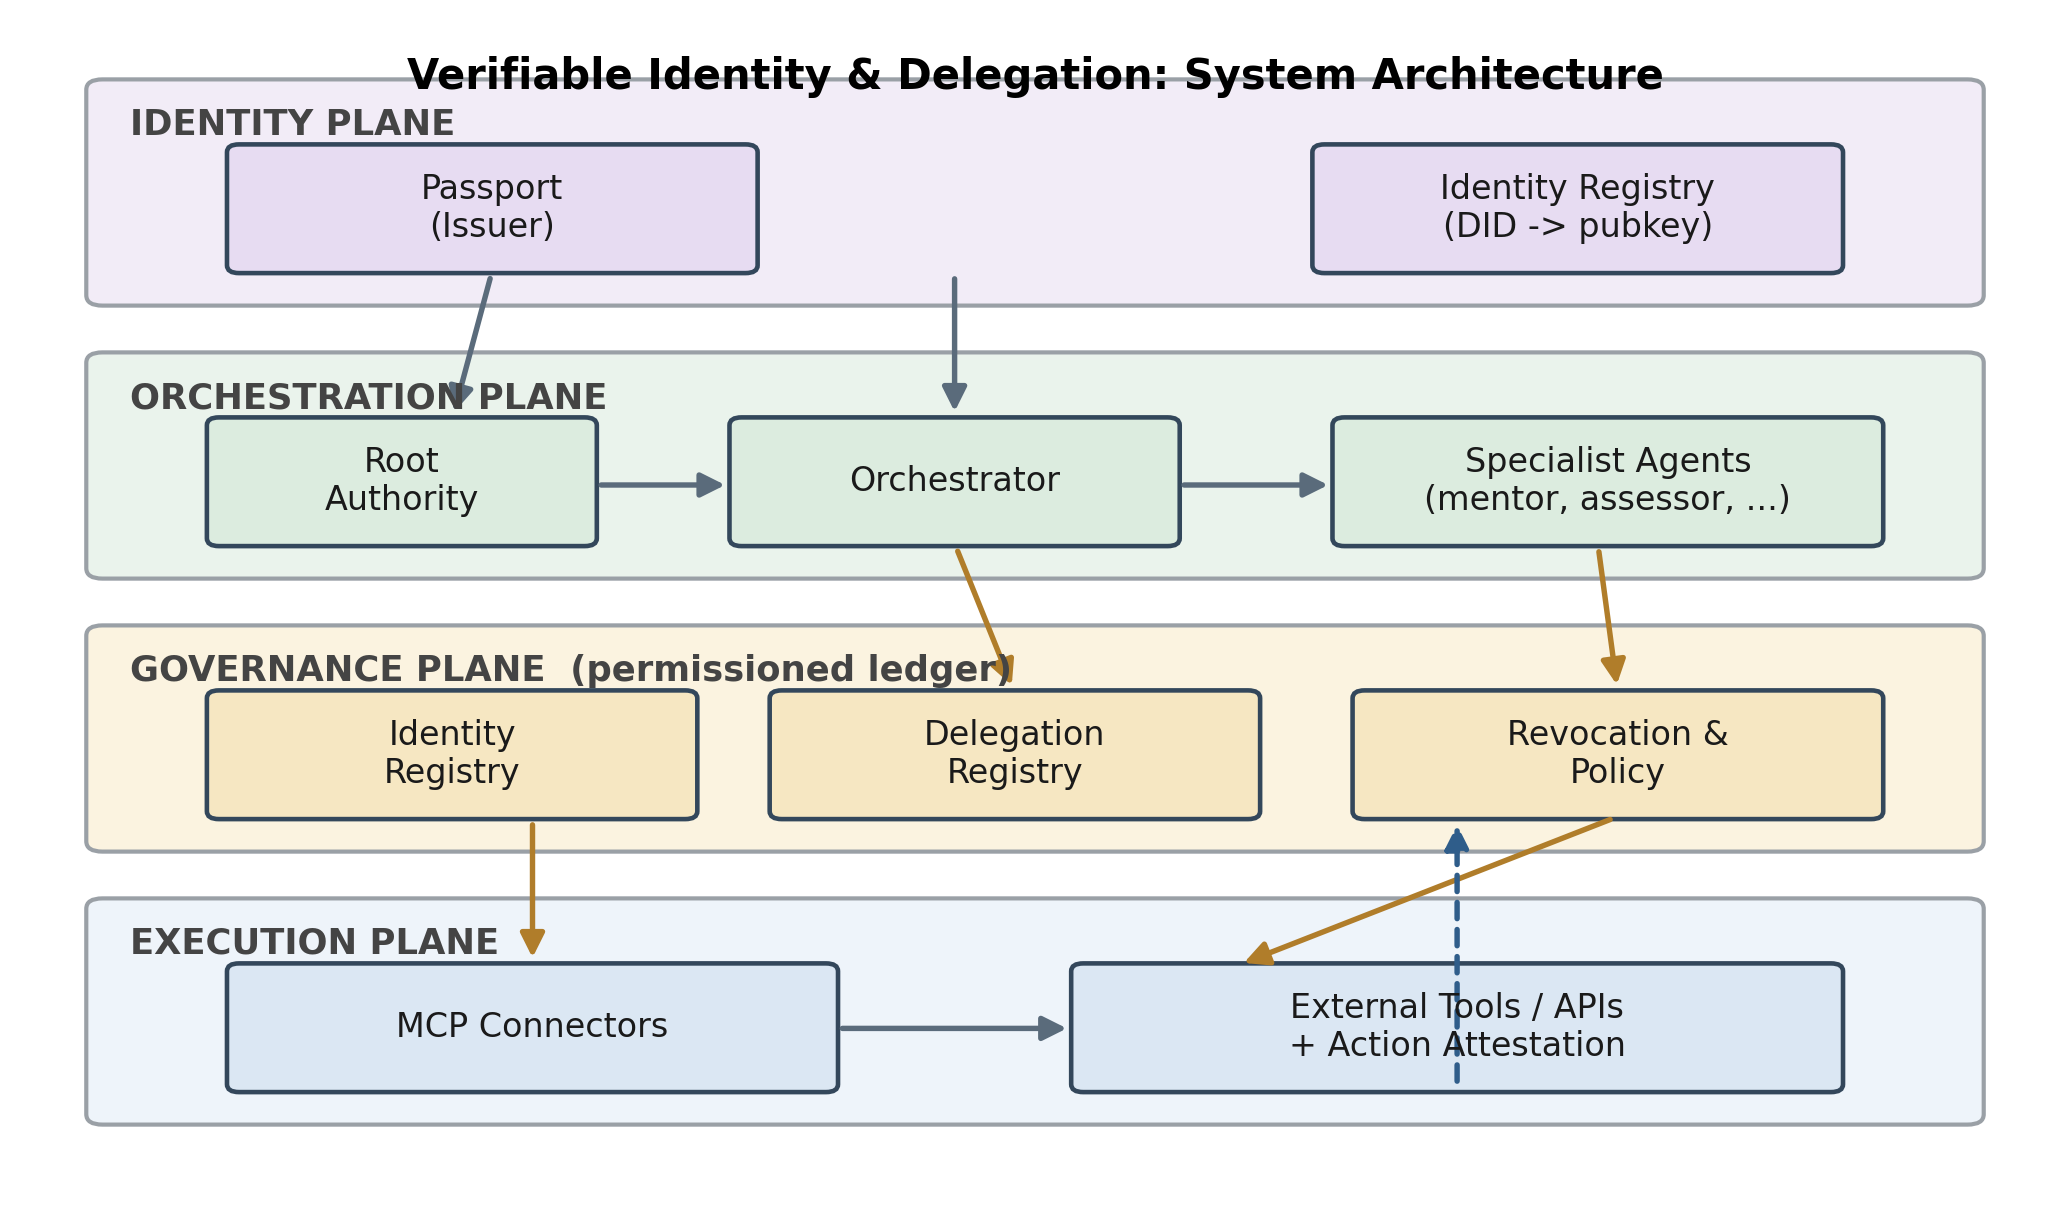
\includegraphics[width=\columnwidth]{fig_arch.png}
\caption{Four-plane architecture: cryptographic identity, orchestrated delegation, on-chain governance, and MCP-mediated execution.}
\label{fig:arch}
\end{figure}

\subsection{Threat Model and Assumptions}
Our adversary may do any of four things: claim another agent's identifier to impersonate it, replay a previously authorized action, attempt an action outside its granted scope, or use a credential that has expired or been revoked. We assume the ledger holds its integrity under an honest majority of endorsing peers, that each agent keeps its private key in a protected store, and that the issuer correctly binds DIDs to public keys. Three threats are out of scope: tampering with an agent's reasoning (prompt injection), compromise of a peer's host, and theft of an agent's private key. A stolen key lets an adversary act as that agent until the corresponding credential is revoked---which is precisely why on-chain revocation and short validity windows matter here. These threats are real and complementary, and we return to them in Section~\ref{sec:concl}.

\subsection{Agent Identity}
Every agent $A$ gets a key pair and a decentralized identifier, written as the tuple in \eqref{eq:id}, where $\mathit{did}_A$ is the identifier and $\mathit{pk}_A$, $\mathit{sk}_A$ are the public and private keys.
\begin{equation}\label{eq:id}
A = \langle\, \mathit{did}_A,\; \mathit{pk}_A,\; \mathit{sk}_A \,\rangle
\end{equation}
The Identity Registry contract stores the binding $\mathit{did}_A \rightarrow \mathit{pk}_A$ along with metadata: the agent's role, its issuer, and its creation time. To verify a message $m$ signed by $A$, the contract resolves $\mathit{pk}_A$ from $\mathit{did}_A$ and checks the signature against it. That is the whole test.

\subsection{Verifiable Delegation Credentials}
When orchestrator $O$ hands work to specialist $S$, it issues a delegation credential $DC$, shown in \eqref{eq:dc}: a signed object that names the issuer and subject DIDs, the permitted scope $\sigma$, a validity window $[t_{nb}, t_{na}]$, and the issuer's signature.
\begin{equation}\label{eq:dc}
DC = \langle\, \mathit{id},\, \mathit{did}_O,\, \mathit{did}_S,\, \sigma,\, [t_{nb}, t_{na}],\, \mathrm{Sign}_{sk_O} \,\rangle
\end{equation}
Credentials compose into a chain. The root authority issues one to the orchestrator, the orchestrator issues a narrower one to a specialist, and scope only ever shrinks as the chain lengthens---it never grows. Each credential's hash is anchored through the Delegation Registry, so the existence, scope, and timing of every grant become immutable and checkable inside the permissioned network. Sensitive payloads can stay off-chain.

\subsection{Smart Contracts and Authorization}
Three contracts handle governance. The Identity Registry resolves and updates DID-to-key bindings. The Delegation Registry records grants and, for any credential, returns the full chain back to a trusted root. The Revocation and Policy contract keeps a revocation list, answers validity-at-time queries, and checks a proposed action against its credential's scope. Each proposed action also carries a fresh nonce $n$ bound into the agent's signature; the contract records consumed nonces, so a captured action cannot be replayed. Authorizing an action $a$ from $S$ is the conjunction in \eqref{eq:auth}: the signature on the action verifies, the nonce is unused, the chain reaches a trusted root, the action sits within scope, the clock falls inside the validity window, and nothing in the chain is revoked. All must hold.
\begin{equation}\label{eq:auth}
\mathrm{Auth}(a,S) = \mathit{Ident} \wedge \mathit{Fresh} \wedge \mathit{Chain} \wedge \mathit{Scope} \wedge \mathit{Valid} \wedge \neg \mathit{Revoked}
\end{equation}
Algorithm~\ref{alg:auth} lays out the check that runs on-chain for every high-impact action.

\begin{algorithm}[t]
\caption{Action Authorization}
\label{alg:auth}
\begin{algorithmic}[1]
\Require $Tx = \{\, \mathit{did}_S,\ \text{action } a,\ \mathit{credId},\ \mathit{nonce}\ n,\ \mathit{sig} \,\}$
\Ensure \textsc{Approve} or \textsc{Reject}
\If{$\neg\,\textsc{VerifySig}(a, \mathit{sig}, \textsc{resolve}(\mathit{did}_S))$}
    \State \Return \textsc{Reject}(``IdentityFailed'')
\EndIf
\If{$\textsc{SeenNonce}(n)$}
    \State \Return \textsc{Reject}(``ReplayedNonce'')
\EndIf
\State $\mathit{chain} \gets \textsc{DelegationRegistry.getChain}(\mathit{credId})$
\If{$\neg\,\textsc{rootIsTrusted}(\mathit{chain})$}
    \State \Return \textsc{Reject}(``BrokenChain'')
\EndIf
\ForAll{$c \in \mathit{chain}$}
    \If{$\textsc{Revoked}(c) \ \lor\ \neg\,\textsc{InWindow}(c, \mathit{now})$}
        \State \Return \textsc{Reject}(``InvalidCredential'')
    \EndIf
\EndFor
\If{$\neg\,\textsc{InScope}(a, \textsc{scopeOf}(\mathit{chain}))$}
    \State \Return \textsc{Reject}(``OutOfScope'')
\EndIf
\State $\textsc{ConsumeNonce}(n)$; \ $\textsc{Ledger.record}(Tx)$; \Return \textsc{Approve}
\end{algorithmic}
\end{algorithm}

\subsection{Execution and Attestation via MCP}
Once an action is approved, it goes to the Execution Plane, where an MCP connector turns it into a concrete tool or API call. When the call finishes, the framework anchors an attestation: the hash in \eqref{eq:att} over the subject DID, the action, the action's nonce, its result, and the identifier of the authorizing chain. This closes the loop. Every external effect is tied permanently to the exact authority it ran under, and the nonce makes that record one-to-one with a single authorized invocation.
\begin{equation}\label{eq:att}
h = H(\, \mathit{did}_S \,\|\, a \,\|\, n \,\|\, \mathit{result} \,\|\, \mathit{chainId} \,)
\end{equation}

\subsection{End-to-End Flow}
Fig.~\ref{fig:flow} walks through one full cycle: the root grants scoped authority, the credential is issued and anchored, the specialist proposes an action, the contracts verify it, MCP executes it, and the result is attested. If verification fails at step~5, the action is blocked and the attempt is logged---so even rejected actions leave a trace.

\begin{figure}[t]
\centering
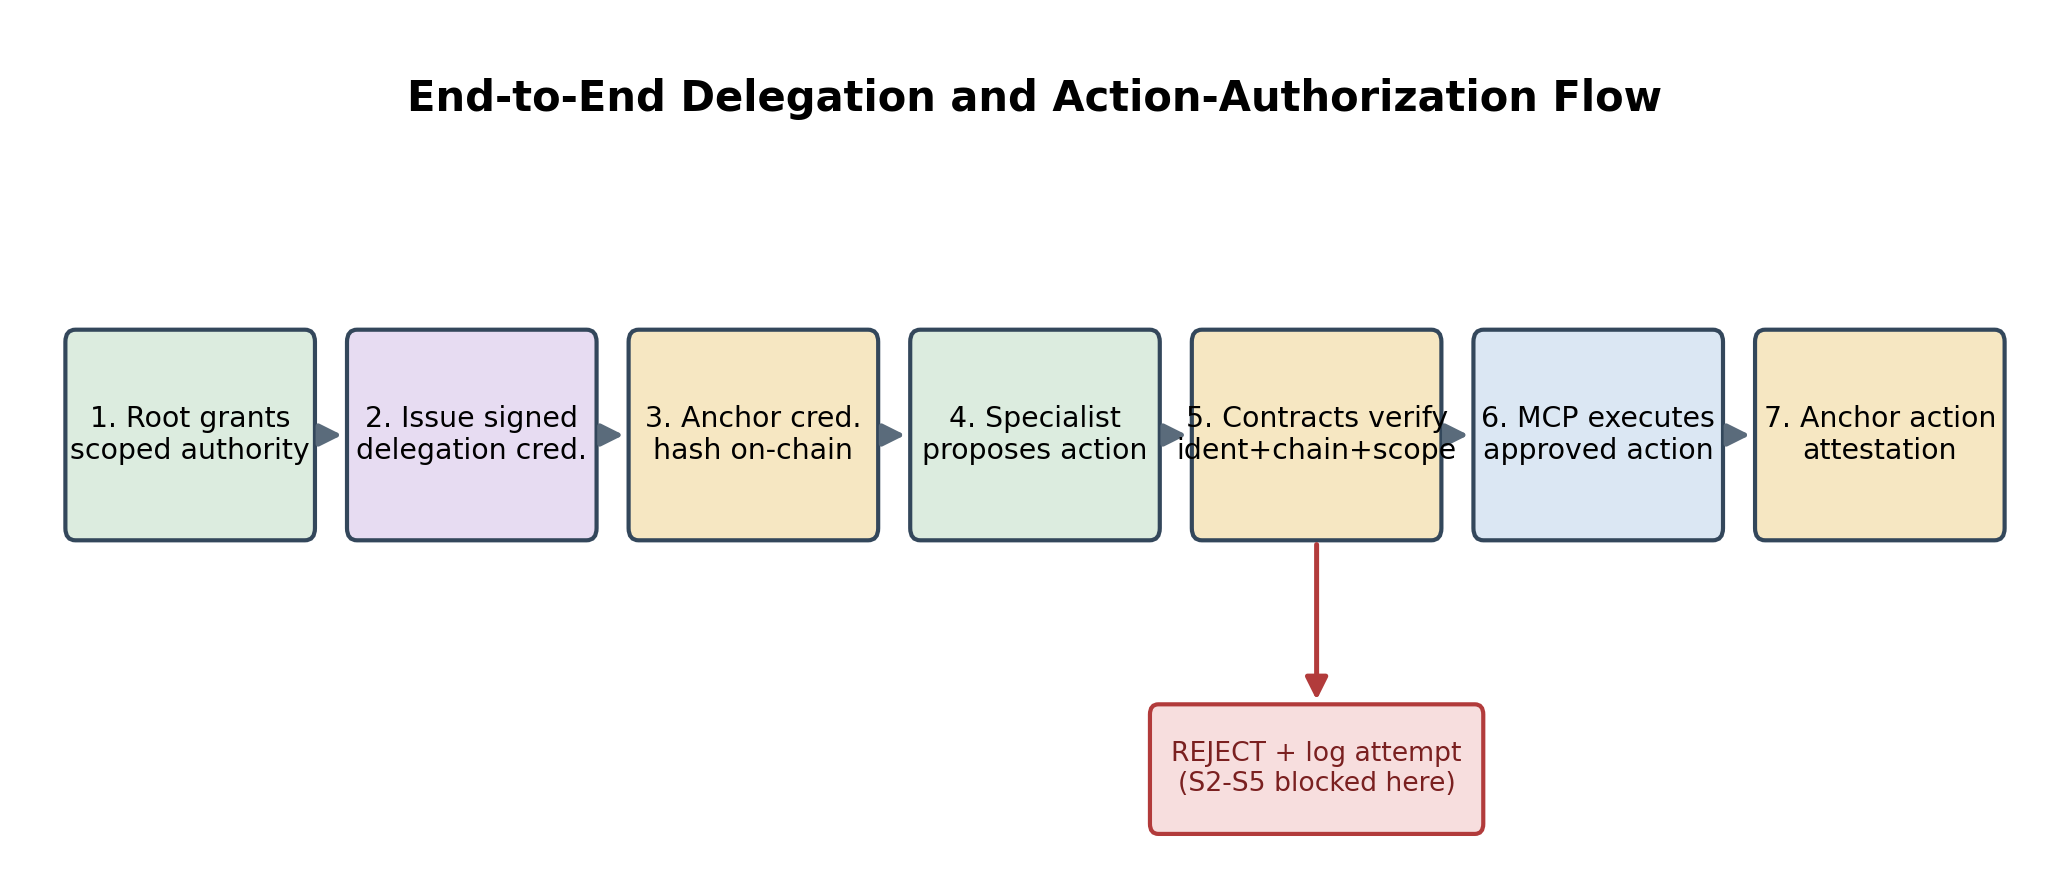
\includegraphics[width=\columnwidth]{fig_flow.png}
\caption{End-to-end delegation and action-authorization flow. Rejected actions are blocked and logged.}
\label{fig:flow}
\end{figure}

\subsection{Worked Example}
Take the banking testbed. The root authority $R$---the account owner or bank---grants the orchestrator $O$ a credential $DC_1$ with scope $\{\textit{assess\_risk}, \textit{screen\_fraud}, \textit{transfer}\}$ over a one-hour window; $O$ in turn grants the risk-assessment specialist $S$ a credential $DC_2$ narrowed to $\{\textit{assess\_risk}\}$. When $S$ proposes an \textit{assess\_risk} action, $\mathrm{Auth}$ verifies $S$'s signature, finds the nonce unused, resolves the chain $[DC_2, DC_1]$ to the trusted root $R$, confirms both credentials are unrevoked and in-window, and checks that \textit{assess\_risk} lies in the effective scope $\{\textit{assess\_risk}\} \cap \{\textit{assess\_risk}, \textit{screen\_fraud}, \textit{transfer}\} = \{\textit{assess\_risk}\}$---so the action runs and an attestation is anchored. If the same $S$ instead proposes a \textit{transfer} action (scenario S3)---moving money it was never authorized to move---every check passes except the last: \textit{transfer} is outside the effective scope, so \textsc{InScope} fails and the action is rejected before it executes. $S$ cannot widen its own authority, because the scope was fixed and signed by $O$ when $DC_2$ was issued.

% =====================================================================
\section{Experimental Setup}\label{sec:exp}
\subsection{Reference Implementation}
In the full framework, the agents and orchestrator are Node.js/Express services with reasoning from the Anthropic API, and governance runs on a Hyperledger Fabric network with the three contracts as chaincode. To measure the authorization layer---the part that is actually new---without the noise of the network and the LLM, we built it as a self-contained Python reference on the cryptography library: Ed25519 identities \cite{rfc8032}, a DID-to-key Identity Registry, signed delegation credentials with scope and validity windows, chain resolution, a revocation registry, a consumed-nonce registry for replay protection, and the $\mathrm{Auth}(\cdot)$ predicate from \eqref{eq:auth}. This isolates exactly the four properties missing from prior work---cryptographic identity, chain verification, scope enforcement, and revocation---and lets us measure their cost and correctness on their own.

\subsection{Measurement Setup}
We measure the two cost components separately and directly. The cryptographic authorization layer---blocking outcomes, chain-reconstruction completeness, per-decision crypto latency, and revocation latency---is measured on the Python reference implementation. The permissioned-ledger ordering and commit latency is measured on a live network: we deployed the three contracts as chaincode on the standard \texttt{fabric-samples} two-organization Hyperledger Fabric~2.5 test-network---a single Raft ordering node, two peer organizations with one peer each, and one certificate authority per organization---and measured the end-to-end submit-to-commit latency of a legitimate authorized action over 500 trials. Because the legacy peer-side chaincode build is incompatible with current Docker Engine releases, the chaincode runs as an external Chaincode-as-a-Service process the peers reach over gRPC; this changes only how the chaincode is launched, not its on-chain logic. End-to-end latency on this network is set by the orderer's batch-cut interval, which we configured to 250~ms with a small batch size (at most two messages per block)---values suited to a latency-sensitive authorization workload, where each consequential action is committed promptly rather than held back to batch for throughput. This interval, not our framework, sets the latency floor; it is a deployment parameter, and the cryptographic cost is unchanged regardless of its value. The crypto testbed mirrors an automated banking platform: an orchestrator delegating to risk-assessment, fraud-screening, and payment specialist agents. We ran the reference implementation on one core of an Intel Core i3-7020U at 2.30~GHz (Windows~10, 12~GB RAM) with Python~3.12 and the cryptography~49.0 library; each enforcement scenario ran 2{,}000 times and each overhead measurement 5{,}000 times. Per-decision crypto latencies are averaged over back-to-back invocations to factor out operating-system scheduling jitter, and we report the means; the 95th-percentile figure is taken from single calls so it still reflects the tail.

\subsection{Baselines}
Three configurations. B0 has no blockchain at all: the orchestrator calls specialists and runs actions through MCP with no on-chain checks. B1 is an allow-list, reproducing the identity model of prior work \cite{jan2025}---an action is authorized if the agent's identifier is on a whitelist. B2 is our DID-plus-delegation framework. B0 shows the cost of adding governance; B1 shows what cryptographic identity and delegation buy over a plain name list.

\subsection{Evaluation Scenarios and Metrics}
Each configuration faces six scenarios: (S1) a legitimate action by a correctly delegated specialist; (S2) an action from an agent presenting a forged identity; (S3) an action outside the granted scope; (S4) an action under a revoked credential; (S5) an action under an expired one; and (S6) a replayed action---a legitimate, already-authorized action captured and resent verbatim. We report four things: how many of the S2--S6 attacks are blocked; whether the full authority chain can be rebuilt from the ledger for every executed action (reconstruction completeness); how long after a revoke the first action is actually blocked (revocation latency); and the overhead---added latency per decision, throughput of the authorization layer, and the measured end-to-end ledger latency.

% =====================================================================
\section{Results and Discussion}\label{sec:res}
\subsection{Security and Correctness}
Table~\ref{tab:sec} gives the enforcement numbers. B0 checks nothing, so it runs every action, including the spoofed, out-of-scope, stale, and replayed ones---0\% blocked. B1 does no better against these attacks: it admits any action that carries a known identifier, and an attacker can simply present a victim's identifier string or resend a captured one, so it too blocks 0\% of S2--S6. B2 blocks all of S2--S6 while letting every legitimate S1 action through, and it rebuilds the full authority chain for 100\% of executed actions. The gap is not a matter of degree. The baselines have no signatures, no scope, no validity windows, no revocation, and no freshness check, so they cannot detect these attacks at all.

\begin{table}[t]
\centering
\caption{Security and Correctness Across Scenarios (measured)}
\label{tab:sec}
\renewcommand{\arraystretch}{1.2}
\begin{tabular}{@{}lccc@{}}
\toprule
\textbf{Scenario / Metric} & \textbf{B0} & \textbf{B1} & \textbf{B2}\\
\midrule
S1 legitimate success (\%)    & 100 & 100 & 100\\
S2 spoof blocked (\%)         & 0   & 0   & 100\\
S3 out-of-scope blocked (\%)  & 0   & 0   & 100\\
S4 revoked blocked (\%)       & 0   & 0   & 100\\
S5 expired blocked (\%)       & 0   & 0   & 100\\
S6 replay blocked (\%)        & 0   & 0   & 100\\
Chain reconstruction (\%)     & 0   & 0   & 100\\
\bottomrule
\end{tabular}
\end{table}

\subsection{Overhead and Scalability}
Table~\ref{tab:over} gives the cost, and Fig.~\ref{fig:res} shows enforcement and latency together. The full $\mathrm{Auth}(\cdot)$ check---verifying the signature, testing the nonce, walking the chain, intersecting scopes, and checking the validity window and revocation list---takes 0.238~ms on average, 0.409~ms at the 95th percentile; the signature check alone is 0.210~ms, and the replay (nonce) check is a hash-set lookup at 0.0003~ms, effectively free. A revoked credential starts being rejected 0.214~ms after the revoke. Set against the measured end-to-end ledger latency---a mean of about 406~ms per action (p95 509~ms) over 500 trials on the Fabric test-network with a 250~ms batch-cut interval---the cryptography adds well under 0.1\% to per-decision latency, which leaves B2's mean decision latency (about 406~ms) indistinguishable from B1's (also about 406~ms). In isolation, the authorization layer itself handles around 4{,}200 verifications per second on one core---well past any realistic rate of agent actions---so the bottleneck is the ledger, not the cryptography, exactly as in \cite{jan2025}. End-to-end throughput rose with offered concurrency as actions filled blocks and then plateaued near 45~tx/s, the point at which the single ordering node and two-peer endorsement saturate. The check is linear in the length of the delegation chain: sweeping the chain from one to ten credentials, each extra credential adds about 3.4~$\mu$s---a revocation-list, validity-window, and scope test---while the one cost that dominates, verifying the action signature, is paid once regardless of depth, since issuer signatures are checked when credentials are anchored rather than at authorization time.

\begin{table}[t]
\centering
\caption{Per-Decision Overhead and Throughput. Crypto rows are measured on the reference implementation; the ledger commit latency is the end-to-end submit-to-commit time measured on the Fabric test-network (250~ms batch-cut interval), a network cost shared by any ledger-anchored design.}
\label{tab:over}
\renewcommand{\arraystretch}{1.2}
\begin{tabular}{@{}lccc@{}}
\toprule
\textbf{Metric} & \textbf{B0} & \textbf{B1} & \textbf{B2}\\
\midrule
Crypto auth, measured (ms)        & 0.0002 & 0.0003 & 0.238\\
Identity verify, measured (ms)    & --     & --     & 0.210\\
Replay (nonce) check, meas.\ (ms) & --     & --     & 0.0003\\
Auth p95, measured (ms)           & 0.0008 & 0.0006 & 0.409\\
Ledger commit, measured (ms)      & -- & 406 & 406\\
Mean decision latency (ms)        & $<$0.01 & 406.1 & 406.4\\
Revocation latency, measured (ms) & --     & --     & 0.214\\
Auth-layer throughput (tx/s)      & $>$10$^6$ & $>$10$^6$ & 4205\\
\bottomrule
\end{tabular}
\end{table}

\begin{figure}[t]
\centering
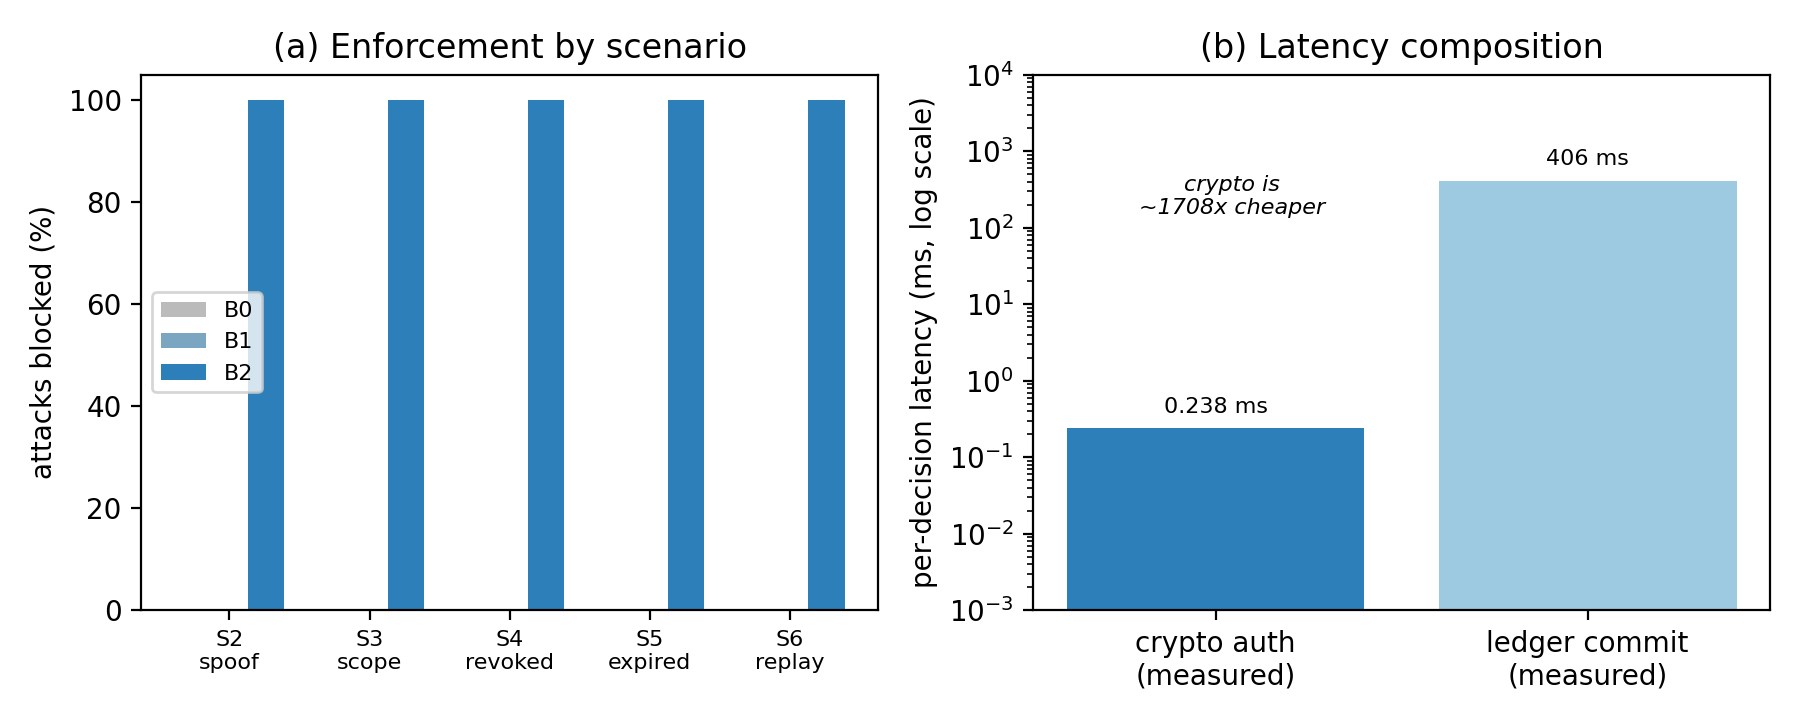
\includegraphics[width=0.86\columnwidth]{results_fig.png}
\caption{Measured enforcement by scenario (a) and per-decision latency composition (b); the crypto authorization is a 0.24~ms sliver atop the measured ledger commit latency (log scale).}
\label{fig:res}
\end{figure}

\subsection{Discussion}
The trade is a negligible cryptographic cost for guarantees that are different in kind. Table~\ref{tab:cap} shows why: only B2 has cryptographic identity, scoped and revocable delegation, and execution-bound auditability at once, and Table~\ref{tab:sec} shows the baselines stop none of the four attacks. What does cost something is the ledger itself, which makes the design a fit for high-impact actions rather than high-frequency, low-stakes calls---a real deployment might route only consequential actions through the chain and let routine ones run directly. The framework has limits worth stating plainly: it trusts the issuer for the first DID-to-key binding, it assumes each agent guards its private key, and it does nothing about an adversary who manipulates an agent's reasoning.

% =====================================================================
\section{Security Analysis}\label{sec:sec}
We take each threat from Section~\ref{sec:fw} and match it to the mechanism that stops it. Table~\ref{tab:threat} summarizes the mapping; the measured blocking rates are in Table~\ref{tab:sec}.

\textit{Identity spoofing (S2).} To act as a victim, an adversary presenting that victim's DID would have to produce a signature over the action that verifies against the victim's registered key. Without the private key, that is infeasible under the EdDSA assumptions \cite{ed25519,rfc8032}, and the \textsc{VerifySig} step in Algorithm~\ref{alg:auth} turns the action away. An allow-list, which checks only that the name is known, cannot tell the two apart.

\textit{Out-of-scope action (S3).} The effective scope is the intersection of scopes down the chain, and intersection can only narrow it from root to leaf. An action whose type is not in that scope fails \textsc{InScope}. Since scope is fixed and signed when the credential is issued, a specialist cannot widen its own authority.

\textit{Revoked and expired authority (S4, S5).} Every credential in the chain is checked against the revocation list and its validity window at execution time, not at issuance. A revoked credential is rejected within 0.22~ms of the revoke, and an expired window fails \textsc{InWindow} every time.

\textit{Replayed action (S6).} A captured action carries a valid signature, an unrevoked credential, and an in-scope request, so the first four checks would pass it. The nonce check is what stops it: the action's nonce is bound into the signature, and the contract records every nonce it consumes, so the second appearance fails \textsc{SeenNonce}. This is the gap a signature-only design leaves open---a valid signature proves authenticity, not freshness---and it is why the conjunction in \eqref{eq:auth} includes a $\mathit{Fresh}$ term. The cost is a single hash-set lookup (0.0003~ms).

\textit{Forged delegation.} Each credential carries its issuer's signature, and we verify it against the issuer's registered key at every link. A fabricated credential whose signature does not check out is rejected, and a chain that fails to terminate at a trusted root returns \textsc{BrokenChain}.

\textit{Auditability.} Because each executed action anchors an attestation \eqref{eq:att} bound to its chain, and every grant is anchored when issued, the complete authority chain rebuilds for 100\% of executed actions---something neither baseline can do. Rejected attempts are logged too, leaving a tamper-evident record of the attacks themselves.

\begin{table}[t]
\centering
\caption{Threats and Defeating Mechanisms}
\label{tab:threat}
\renewcommand{\arraystretch}{1.3}
\begin{tabular}{@{}p{1.6cm}p{4.0cm}c@{}}
\toprule
\textbf{Threat} & \textbf{Defeating mechanism} & \textbf{Scenario}\\
\midrule
Identity spoofing   & Ed25519 signature over action vs. registered DID key & S2\\
Out-of-scope action & Scope intersection along delegation chain            & S3\\
Revoked authority   & On-chain revocation list checked per credential      & S4\\
Expired authority   & Validity-window $[t_{nb}, t_{na}]$ check at execution & S5\\
Replayed action     & Per-action nonce, consumed on first use              & S6\\
Forged delegation   & Issuer signature verified for every credential       & S2--S6\\
\bottomrule
\end{tabular}
\end{table}

% =====================================================================
\section{Conclusion and Future Work}\label{sec:concl}
We have described a blockchain-anchored framework that gives orchestrated AI agents real cryptographic identity and ties every delegated action to a scoped, revocable authority chain---checked before the action runs and reconstructable after it, through an MCP execution layer. The implementation of the authorization layer blocks all of the spoofed, out-of-scope, revoked, expired, and replayed actions that the no-blockchain and allow-list baselines wave through, rebuilds the full authority chain for every executed action, and costs just 0.24~ms of cryptographic work per decision---negligible next to the measured ledger commit latency of about 406~ms. This fills a gap in earlier agentic-governance work, which still identifies agents by allow-list and models neither delegation nor revocation. We deployed the contracts on a Hyperledger Fabric~2.5 network and confirmed end-to-end that the cryptographic overhead vanishes against ordering and commit, so the bottleneck is the ledger rather than the authorization. Reducing that ledger latency further---through a faster ordering service or hardware---and evaluating delegation across organizational ledgers, on-chain reputation that weights authority by behavior, zero-knowledge proofs of authority for privacy, and formal verification of the authorization protocol remain future work.

% =====================================================================
\section*{Use of AI Assistance}
In preparing this work the author used an AI assistant (a large language model) to help edit prose, scaffold and debug the reference implementation, and cross-check the references. All technical claims, the framework design, the experiments, and the reported results were checked by the author, who takes full responsibility for the content. The measured numbers were produced by executing the reference implementation and the Hyperledger Fabric network benchmark; none were generated by the AI assistant.

% =====================================================================
\bibliographystyle{IEEEtran}
\bibliography{references}

\end{document}
